\chapter{Results and Discussions}

\section{Experimental Analysis on GSM8k datset}

The GSM8k dataset stands as a gold standard for evaluating the proficiency of LLMs in solving grade-school math word problems. Comprising 8,500 high-quality, linguistically diverse problems, this dataset encompasses a wide array of mathematical concepts, including arithmetic, fractions, percentages, and basic algebra. The problems are carefully designed to require multi-step reasoning, mirroring the complexity of real-world mathematical challenges.\\
\\
Unlike traditional math datasets that often focus on simple calculations, GSM8k emphasizes the understanding of natural language and the ability to translate word problems into a sequence of mathematical operations. This unique characteristic makes it a particularly challenging yet highly relevant benchmark for assessing the mathematical reasoning abilities of LLMs.\\
\\
The evaluation of LLMs on the GSM8k dataset, facilitated by the DSPy framework, offers a comprehensive understanding of their strengths and weaknesses in this critical domain. By leveraging DSPy's streamlined evaluation pipeline, we were able to conduct a rigorous and reproducible analysis of model performance, uncovering nuanced insights into their mathematical reasoning capabilities.\\
\\
The evaluation of various large language models (LLMs) on the GSM8k dataset, facilitated by the DSPy framework, reveals nuanced differences in their mathematical reasoning abilities. Utilizing DSPy's streamlined evaluation tools, we analyzed model performance across varying model architectures and test data sample sizes. Below are the key findings:


\begin{table*}[t]
\centering
\begin{tabular}{\salinewidth}{lc|ccc}
\toprule
               & \textbf{Number of}           & \multicolumn{4}{c}{``dspy COT''} \\
\textbf{Model} & \textbf{Questions} & \textbf{Accuracy (Sample 1)$\uparrow$} & \textbf{Accuracy (Sample 2)$\uparrow$} & \textbf{Avg Accuracy $\uparrow$} & \textbf{Accuracy Delta $\uparrow$}\\
\toprule

Mistral-7B &  50 &   0.32 & 0.40 & 0.36 & 0.08\\
Mistral-7B &  100 &   0.33 & 0.40 & 0.36 & 0.07\\
Mistral-7B &  150 &   0.31 & 0.34 & 0.32 & 0.03\\
Mistral-7B & 200 &   0.28 & 0.32 & 0.30 & 0.04\\

\midrule
Mixtral-8x7B &  50 &   0.58 & 0.54 & 0.56 & 0.04\\
Mixtral-8x7B &  100 &   0.58 & 0.60 & 0.59 & 0.02\\
Mixtral-8x7B &  150 &   0.55 & 0.54 & 0.54 & 0.01\\
Mixtral-8x7B & 200 &   0.55 & 0.54 & 0.54 & 0.01\\

\midrule
Llama2-13B &  50 &   0.26 & 0.28 & 0.27 & 0.02\\
Llama2-13B &  100 &   0.24 & 0.31 & 0.27 & 0.07\\
Llama2-13B &  150 &   0.23 & 0.27 & 0.25 & 0.04\\
Llama2-13B & 200 &   0.23 & 0.25 & 0.24 & 0.02\\

\midrule
Llama2-70B &  50 &   0.50 & 0.50 & 0.50 & 0.00\\
Llama2-70B &  100 &   0.47 & 0.55 & 0.51 & 0.08\\
Llama2-70B &  150 &   0.43 & 0.51 & 0.47 & 0.08\\
Llama2-70B & 200 &   0.41 & 0.47 & 0.44 & 0.06\\

\midrule
Llama3-8B &  50 &   0.74 & 0.72 & 0.73 & 0.02\\
Llama3-8B &  100 &   0.70 & 0.72 & 0.71 & 0.02\\
Llama3-8B &  150 &   0.69 & 0.73 & 0.71 & 0.04\\
Llama3-8B & 200 &   0.65 & 0.71 & 0.68 & 0.06\\

\midrule
Llama3-70B &  50 &   0.84 & 1.00 & 0.92 & 0.16\\
Llama3-70B &  100 &   0.85 & 0.94 & 0.89 & 0.09\\
Llama3-70B &  150 &   0.85 & 0.94 & 0.89 & 0.09\\
Llama3-70B & 200 &   0.85 & 0.93 & 0.89 & 0.08\\

\bottomrule
\end{tabular}
\vspace{2mm}
\caption{Performance results for the prompts generated by dspy COT module}
\vspace{-5mm}
\label{table:optimized-performance}
\end{table*}



\begin{enumerate}
    \item \textbf{DSPy-Powered Evaluation:} By harnessing the capabilities of DSPy, we established a standardized and reproducible evaluation process. This ensured that all models were subjected to the same testing conditions, allowing for a fair and objective comparison of their mathematical prowess.

    \item \textbf{Performance Trends:} DSPy's analysis revealed distinct performance trends. Larger models, exemplified by Meta-Llama-3-70B-Instruct as shown in Figure \ref{bar_1} and \ref{box_1}, consistently outperformed their smaller counterparts. This observation, enabled by DSPy's meticulous data collection and aggregation, reinforces the notion that model scale is a critical factor in mathematical reasoning tasks.

    \begin{figure}
    \centering
    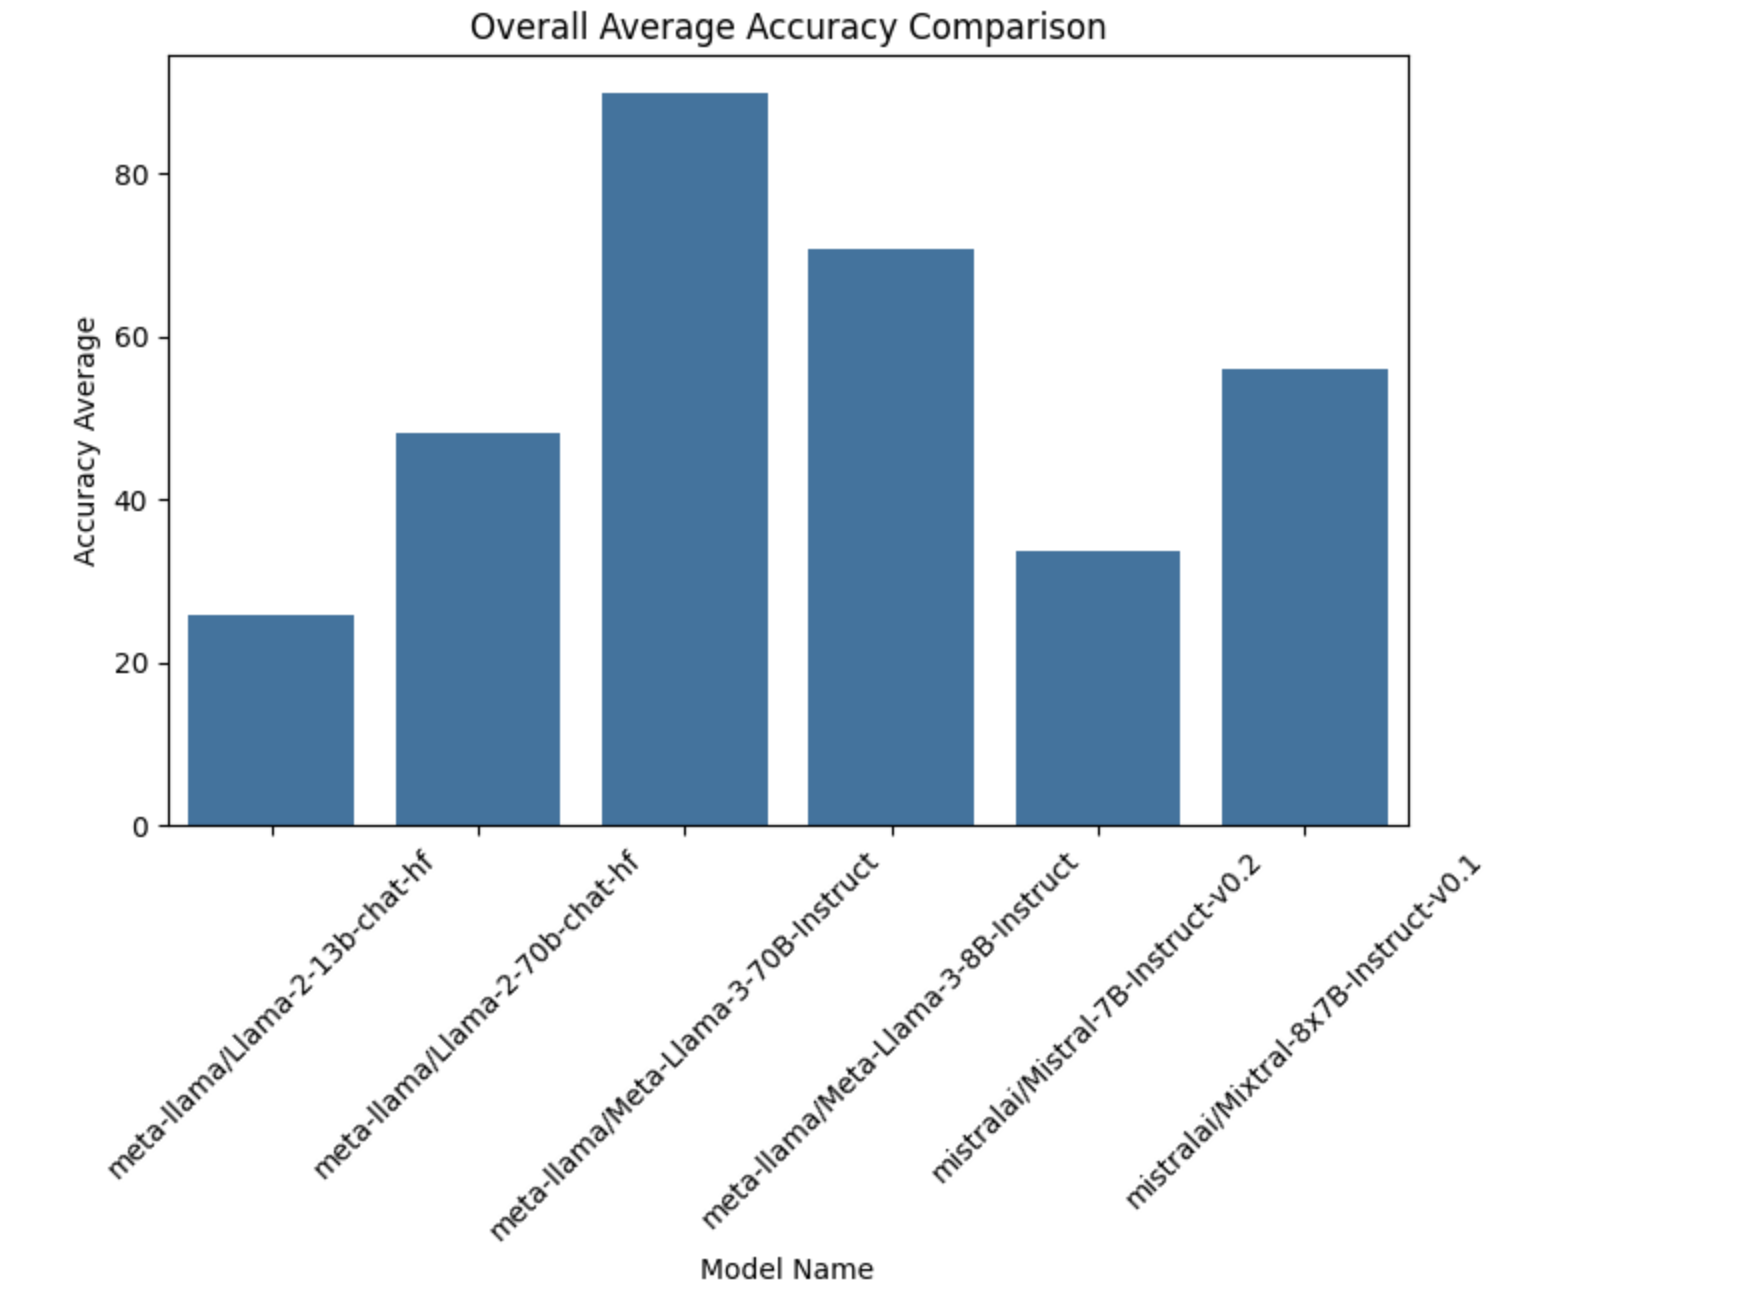
\includegraphics[width=\textwidth,]{report_template/images/bar_1.png}
    \caption{Bar plot comparing average accuracy of two sets of test data from GSM8K dataset across different language models.}
    \label{bar_1}
    \end{figure}

    \begin{figure}
    \centering
    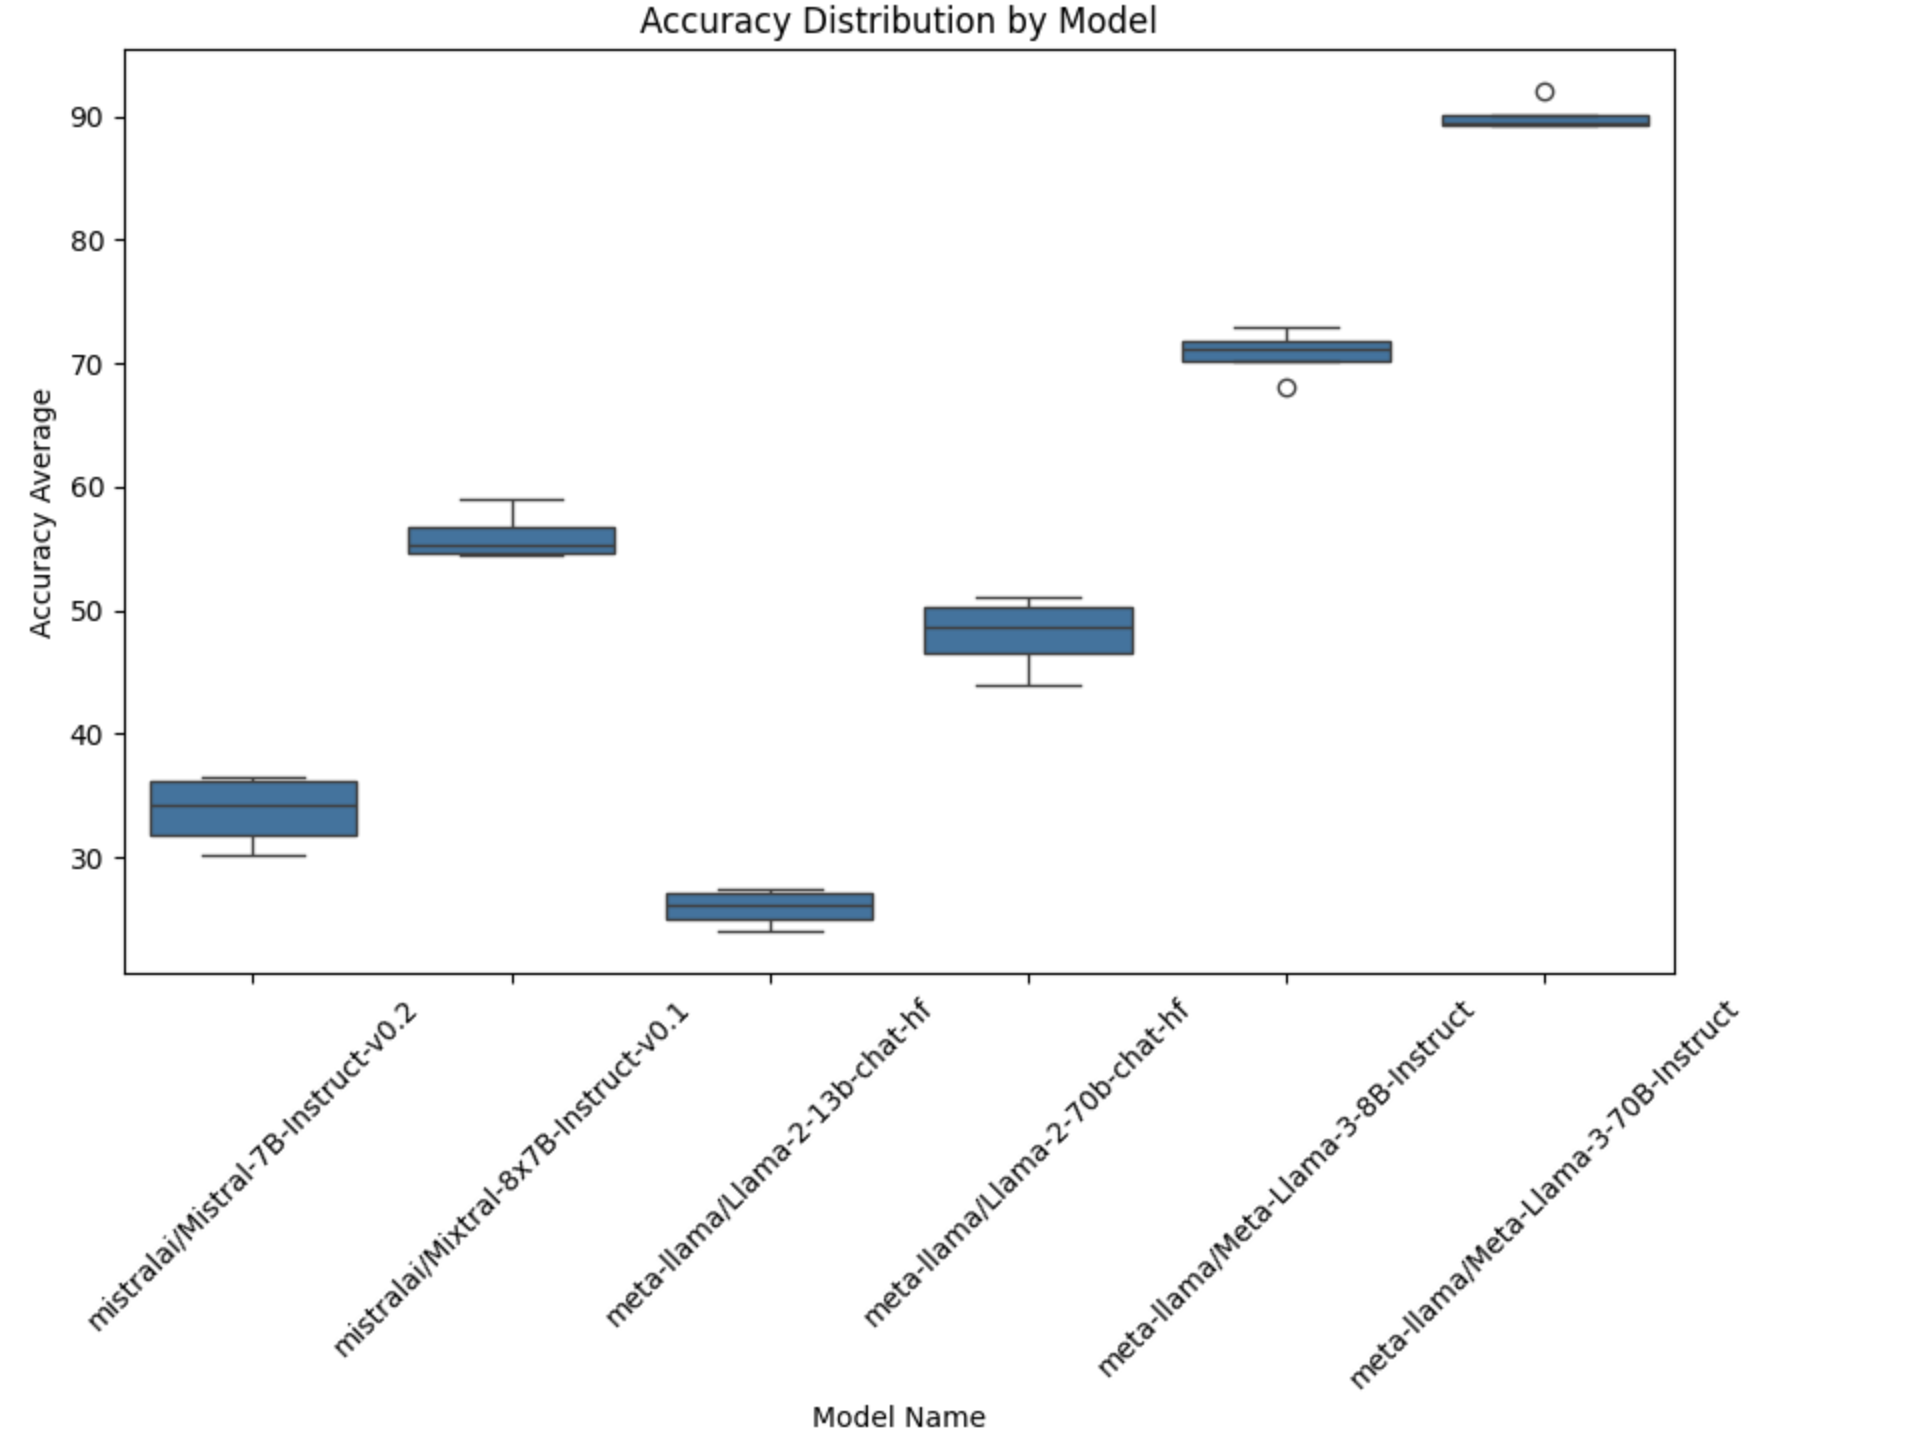
\includegraphics[width=\textwidth,]{report_template/images/box_1.png}
    \caption{Bar plot comparing average accuracy of two sets of test data from GSM8K dataset across different language models.}
    \label{box_1}
    \end{figure}

    \item \textbf{Sample Size Sensitivity Unveiled:} The utilization of DSPy's flexible evaluation pipeline allowed us to investigate the impact of test data sample size. The analysis showed a subtle but consistent decrease in accuracy as the sample size increased as shown in Figure \ref{line_1}, indicating potential challenges in model generalization and robustness to data variations.

    \begin{figure}
    \centering
    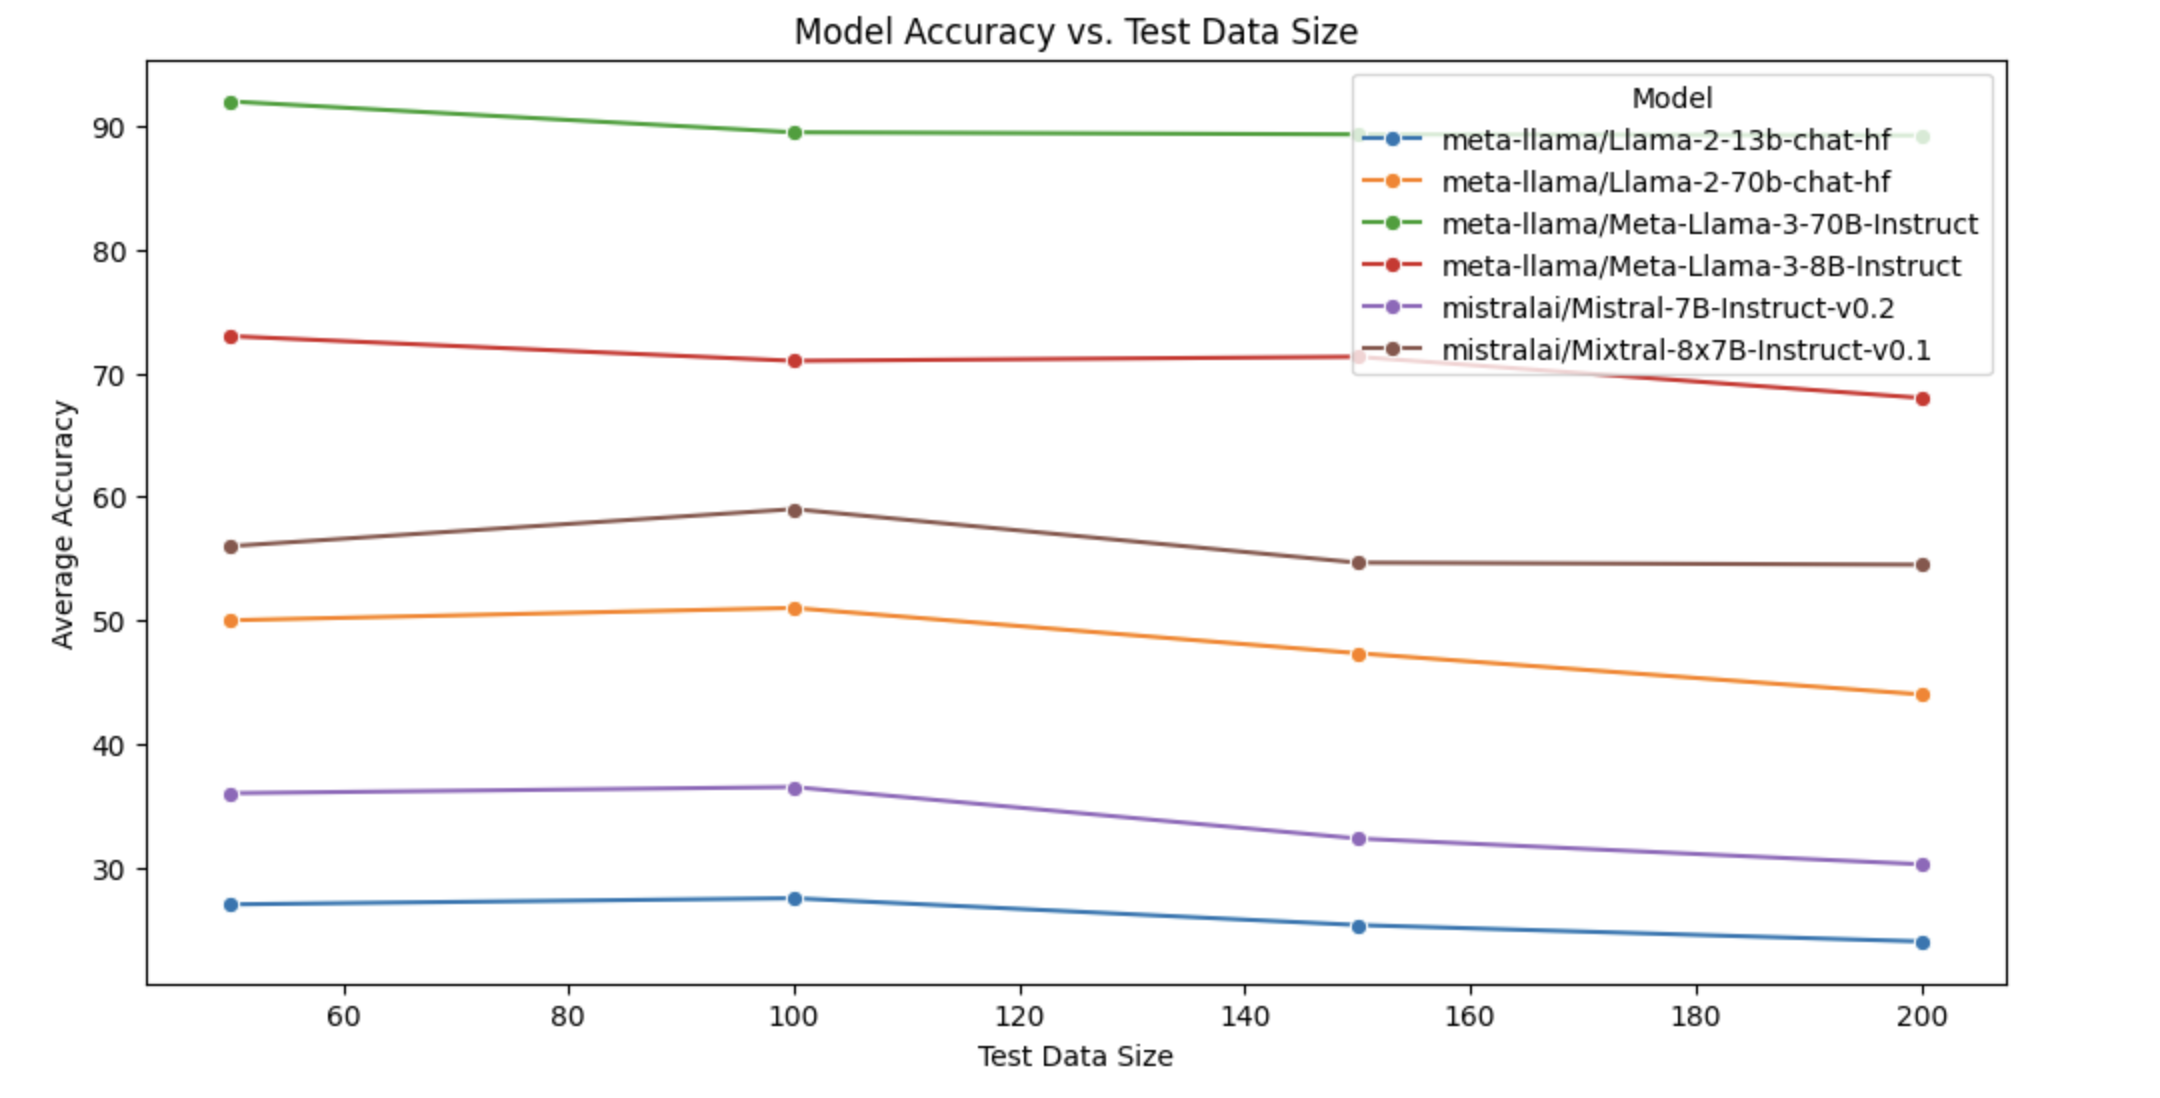
\includegraphics[width=\textwidth,]{report_template/images/line_1.png}
    \caption{Bar plot comparing average accuracy of two sets of test data from GSM8K dataset across different language models.}
    \label{line_1}
    \end{figure}

    \item \textbf{The Power of Instruction Fine-Tuning:} Through DSPy's comprehensive evaluation, we observed a clear advantage for models fine-tuned with instruction data. The inclusion of task-specific instructions during training, as facilitated by DSPy's seamless integration with various fine-tuning techniques, significantly enhanced model performance.

    \item \textbf{Accuracy Fluctuations Detected:} DSPy's fine-grained analysis revealed interesting fluctuations in model accuracy across different data samples, particularly for smaller models. This finding, made possible by DSPy's ability to conduct multiple evaluations and aggregate results, emphasizes the importance of robust evaluation strategies for accurately assessing LLM capabilities.
\end{enumerate}